\chapter{Teoretická část}
\section{Suspendace}
Smyslem suspendace v~mechanicky míchaných nádobách je udržení pevných částic ve vznosu tak, aby došlo ke zintenzivnění transportu hmoty a tepla mezi kapalinou a pevnou fází. Pro dosažení tohoto stavu je třeba systému dodat energii v~podobě mechanické práce. K~vykonání této práce se používají rozmanité typy mechanických míchadel, které jsou voleny podle konkretního charakteru dané úlohy. Dodaná energie poté vede k~vytvoření turbulentního proudění, jenž uvede částice pevné fáze do vznosu a následně je rozptýlí v~kapalině. Nutnou podmínkou pro zajištění tohoto vznosu je potřeba, aby výsledná vertikální složka síly působící na částici byla větší než tíhová síla zmenšená o~sílu vztlakovou. Menší částice jejichž hustota je přibližně rovna hustotě kapalina se po dosažení suspenzních podmínek pohybují společně s~kapalinou. Při nižších koncentracích pevné fáze se toto proudění chová spíše jako jednofázový tok. Naopak rychlost pohybu těžších částic se liší od rychlosti kapalné fáze, jenž musí na pevnou fázi působit větší silou k~zabránění jejímu usazování. Výslednou kvalitu vzniklé suspenze ovlivňuje řada faktorů, kde mezi nejvýznamnější patří fyzikální vlastnosti, jak kapalné, tak pevné fáze, provozní podmínky a geometrie systému a míchadla.

\subsection{Stupně suspendace}
Nároky na homogenitu vsádky se liší dle konkretních provozních požadavků. Jedním z~pojmů, který se používá k~popisu míry homogenizace vsádky v~mechanicky míchaných nádobách je stupeň suspendace. Obecně se rozlišují tři stupně suspendace: částečná, úplná a homogenní (obr. \ref{fig:typsus}). 
  
\begin{figure}[h!]
  \centering
  \subfloat[Částečná]{\label{fig:typ1}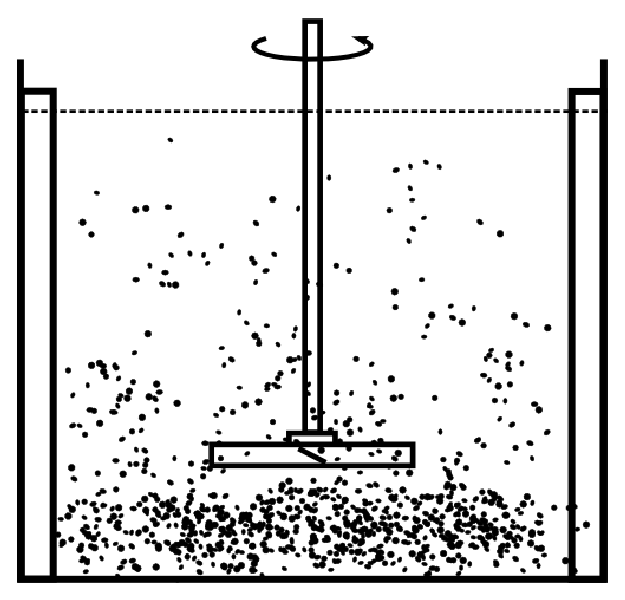
\includegraphics[scale=0.35]{images/typy_suspenzi-1.eps}}
  \qquad
  \subfloat[Úplná]{\label{fig:typ2}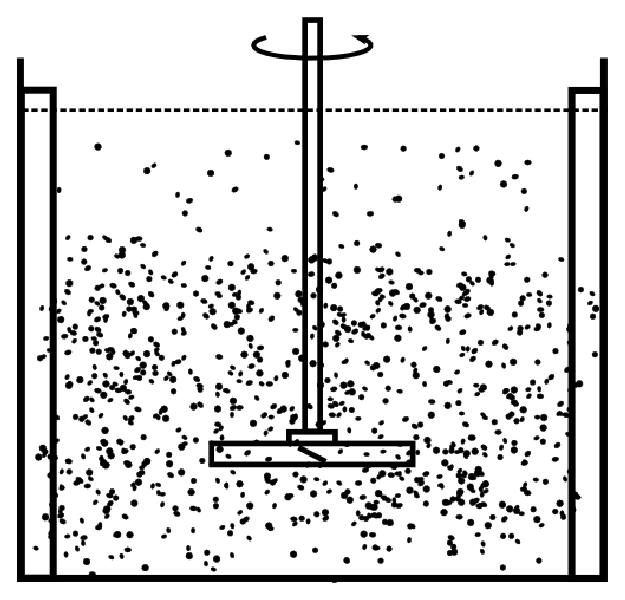
\includegraphics[scale=0.35]{images/typy_suspenzi-2.eps}}
  \qquad
  \subfloat[Homogenní]{\label{fig:typ3}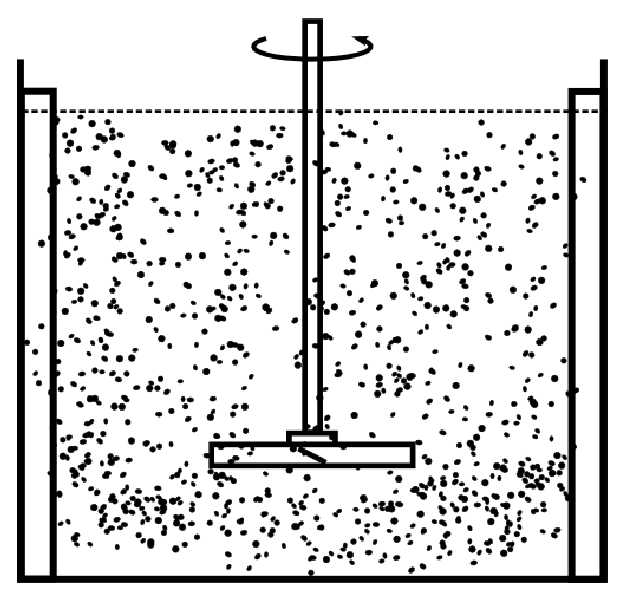
\includegraphics[scale=0.35]{images/typy_suspenzi-3.eps}}
  \caption{Stupně suspendace}
  \label{fig:typsus}
\end{figure}

Při částečné suspendaci lze vizuálně pozorovat pohyb částic pevné fáze pouze v~blízkosti dna nádoby. Toto shlukování má za následek zhoršení přestupu tepla a hmoty, což v~důsledku může snížit rychlost probíhajících chemických reakcí. Z~výše uvedeného vyplývá, že podmínky částečné suspendace jsou postačují pouze při míchaní vysoce rozpustných látek.

Stav úplné suspendace je charakterizován pohybem pevné fáze v~celé nádobě, přičemž žádná částice nezůstává na dně déle než jednu až dvě sekundy. Tato podmínka se někdy označuje jako Zwieteringovo kritérium podle autora, který jako první na základě experimentů navrhl vztah k~výpočtu kritické (minimální) frekvence otáčení míchadla potřebné k~dosažení stavu úplné suspendace. Při tomto stavu je maximální povrch částic vystaven kapalině, což má za následek intenzivní transport hmoty a tepla mezi jednotlivými fázemi.

Posledním stádiem je dosažení stavu homogenní suspendace, při němž částice pevné fáze dosahují prakticky rovnoměrného rozložení v~celém promíchávaném systému. Jakékoliv další zvýšení frekvence míchadla nebo jeho příkonu nemá již prakticky žádný vliv na distribuci pevné fáze. Dosažení stavu homogenní suspendace je často důležité u~procesů, které vyžadují rovnoměrné rozložení částic v~systému. Příkladem takovéhoto procesu může být krystalizace, kde nerovnoměrná koncentrace pevné fáze způsobuje tvorbu míst s~lokálním přesycením, jenž následně negativně ovlivňují kvalitu vzniklých krystalů. Nicméně ve většině případů je postačující dosažení stavu úplné suspendace, který vyžaduje menší množství vykonané práce.

\subsection{Kritická frekvence otáčení míchadla}
Jak již bylo zmíněno v~předcházející kapitole, kritická frekvence otáčení je minimální rychlost otáčení míchadla potřeba k~udržení částic pevné fáze ve vznosu. První kdo navrhl empirickou korelaci k~jejímu výpočtu byl \citet{zwi58}. Jím navržený vztah má tvar:
\begin{equation}
	N_{js} = \left[\frac{g(\rho_{s}-\rho_{l})}{\rho_{l}}\right]^{\num{0.45}}W^{\num{0.13}}d_{p}^{\num{0.2}}D^{\num{-0.85}}\nu^{\num{0.1}}S
	\label{eq:nkrit}
\end{equation} 

\noindent kde $g$ je gravitační zrychlení, $\rho_{s}$ hustota pevné fáze, $\rho_{l}$ hustota kapalné fáze, $W$ relativní hmotnostní zlomek pevné fáze, $d_{p}$ průměr částice pevné fáze, $\nu$ kinematická viskozita a $S$ je bezrozměrná Zwieteringova konstanta, která zohledňuje geometrii systému a míchadla (tab. \ref{tab:S}). Ze vztahu je dobře patrné, že rozdíl hustot jednotlivých fází nejvýznamněji ovlivňuje výslednou kritickou frekvenci otáčení míchadla. Později provedené studie \citep{nie68,bal78,chou97} obecně potvrdily platnost Zwieteringova vztahu. Nicméně \citet{chou97} experimentálně ukázal, že při koncentraci pevné fáze menší než \volproc{2} nebo větší než \volproc{15} se již tato korelace jeví jako nepříliš spolehlivá.

\begin{table}[h!]
\begin{center}
\caption{Zwieteringovy konstanty pro \SI{45}{\degree} PBT}
\label{tab:S}
\begin{tabular}{llr}
\toprule
Šířka lopatky & Světlá výška & Hodnota \\
\midrule

$D/\num{3.5}$ \\
& $T/4$ & \num{4.8} \\
& $T/6$ & \num{4.6} \\
& $T/8$ & \num{3.2} \\
$D/4$ \\
& $T/4$ & \num{4.4} \\
& $T/6$ & \num{4.1} \\
& $T/8$ & \num{3.7} \\

\bottomrule
\end{tabular}
\end{center}
\end{table}

\subsection{Kvalita suspenze (stupeň homogenizace)}
Další užitečnou charakteristikou systému kapalina-pevná fáze je takzvaná kvalita suspenze, což je směrodatná odchylka koncentrace pevné fáze. Často se však dává přednost vyjádření pomocí objemového zlomku pevné fáze. Pro konečný počet $n$ měření lze kvalitu suspenze definovat jako:
\begin{equation}
	\sigma = \sqrt{\frac{1}{n}\sum_{i=1}^{n}\left(\frac{c_{i}}{\bar{c}} - 1\right)^{2}}
	\label{eq:kvasus}
\end{equation}  

\noindent Díky své diskrétní povaze je tato veličina navíc dobře stanovitelná pomocí simulační techniky CFD. S~rostoucí homogenitou systémů číselná hodnota kvality suspenze klesá a v~limitním případě je nulová. Někdy se proto místo kvality suspenze používá pojem stupeň homogenizace, jenž vznikne odečtením kvality suspenze od jedničky.

\citet{boh80} určili na základě experimentů hodnoty kvality suspenze pro jednotlivé stupně suspendace. Jejich výsledky jsou shrnuty v~tab. \ref{tab:kvasus}.

\begin{table}[h!]
\begin{center}
\caption{Rozdělení stupňů suspendace dle kvality suspenze}
\label{tab:kvasus}
\begin{tabular}{cc}
\toprule
Stupeň suspendace & Kvalita suspenze \\
\midrule

Částečná &  $\sigma \geq \num{0.8}$ \\
Úplná & $\num{0.2} < \sigma < \num{0.8}$ \\
Homogenní & $\sigma \leq \num{0.2}$ \\

\bottomrule
\end{tabular}
\end{center}
\end{table}

\subsection{Výška vznosu pevné fáze}
Při míchaní suspenzní se ve vsádce tvoří snadno rozlišitelná oblast ve které se vyskytuje naprostá většina částic pevné fáze. Vzdálenost mezi dnem nádoby a rozhraním této oblasti se někdy také nazývá jako výška suspenzního mraku. 

Experimentálně studovali výšku suspenzního mraku např. autoři \citet{hic97}. Z~jejich měření vyplynulo, že nejvýznamnější vliv na výšku vznosu pevné fáze má poměr průměrů míchadla a nádoby $(D/T)$, poměr světlé výšky a průměru nádoby $(C/T)$ a koncentrace pevné fáze. Dosažení dobré distribuce částic ve vysoké nádobě $(H > T)$ se ukázalo jako poměrně problematické, a proto výzkumníci zdůraznili potřebu použití více míchadel v~takovýchto systémech.

\citet{bit02} odvodili korelaci pro výpočet výšky suspenzního mraku na základě dostupných experimentálních dat, které naměřili \citet{hic97} a \citet{buj99}. Zmíněný vztah byl navržen pro rychloběžná axiální míchadla a má tvar:
\begin{equation}
	C_{H}=\frac{N}{N_{js}}\left[\num{0.84} - \num{1.05}\frac{C}{T} + \num{0.7}\frac{(D/T)^{2}}{1 - (D/T)^{2}}  \right]T
	\label{eq:sushei}
\end{equation}  

\subsection{Doba homogenizace}
Doba homogenizace $t_{mix}$ je definována jako čas potřebný k tomu, aby se hodnota normalizované koncentrace stopovací látky $c(t)^{*}$ pohybovala v předem zvoleném rozmezí. Nejčastěji se volí přípustná hodnota fluktuace \SI{\pm 5}{\percent}, tedy $c(t)^{*} \in \left<\num{0.95};\num{1.05}\right>$. 

Výše zmíněná normalizovaná kocentrace je určena vztahem:
\begin{equation}
	c(t)^{*} = \frac{c(t) - c_{0}}{c_{\infty} - c_{0}}
	\label{eq:bezkon}
\end{equation}

\noindent přičemž $c(t)$ je koncentrace stopovací látky v čase $t$, $c_{\infty}$ je koncentrace ve vsádce po dokonalém rozmíchání a $c_{0}$ představuje počáteční koncentraci v systému.  

Hodnota doby homogenizace také velmi záleží na místě měření zmíněné koncentrace. Například \citet{buj99} měřili dobu homogenizace pro systém kapalina-pevná fáze v mechanicky míchané nádobě. Z výsledků vyplynulo, že nad suspenzním mrakem je doba homogenizace přibližně dvacetkrát delší než v oblasti, která je bohatá na přítomnost částic pevné fáze.

%\newpage 
\section{Počítačová dynamika tekutin (CFD)}
Následující kapitola obsahuje stručný přehled základních rovnic a matematických modelů, které jsou uplatněny při simulaci pomocí techniky CFD. Hlavní důraz je kladen na problematiku isotermního vícefázového proudění kapalina-pevná fáze v mechanicky míchaných nádobách.

\subsection{Úvod do CFD}
Počítačová dynamika tekutin (angl. computational fluid dynamics -- CFD) je jedno z odvětví hydromechaniky, jenž využívá numerické metody a algoritmy k řešení problémů zahrnující proudění tekutin, transport hmoty a tepla, chemické reakce a celou řadu dalších fyzikálně-chemických jevů. Na počátku každé CFD simulace je třeba nejprve vytvořit model zkoumaného systémů na který jsou následně aplikovány matematické postupy tak, aby byly ze zadaných okrajových a počátečních podmínek získány vybrané údaje o dějích probíhajících v celé zkoumané doméně při respektování fyzikálních zákonů. Tyto zákony jsou nejčastěji formulovány v podobě parciálních diferenciálních rovnic. 

S prudkým nárůstem výkonu výpočetní techniky se metoda CFD stala přístupnější širšímu množství uživatelů. Mezi její hlavní výhody patří schopnost studovat systém za podmínek, kdy experimentální měření jsou těžko proveditelná, či přímo nemožná. Díky tomu je možné např. dosáhnout znatelného snížení finančních a časových nákladů ve vývojové fází nového výrobku. Nicméně je třeba dodat, že každý simulační výpočet je silně závislý na dodaných počátečních a okrajových podmínkách, a proto CFD nikdy nemůže úplně nahradit experimentální měření.

Celou CFD simulaci lze rozdělit do třech hlavních kroků: tvorba geometrie a výpočetní sítě, vlastní výpočet a analýza výsledků

\subsubsection{Tvorba geometrie a výpočetní sítě (preprocessing)}
V první fází je vytvořena geometrie zkoumaného systému, která je následně rozdělena na konečný počet kontrolních objemů (buněk). Vzniklá výpočetní síť může obsahovat buňky různých typů. Dvojrozměrná doména se nejčastěji dělí na trojúhelníky nebo obdélníky. V trojrozměrném případě se nejčastěji využívají jehlany, hranoly, kvádry či další mnohostěny. V současnosti se již dává přednost nestrukturovaným sítím před strukturovanýma. Pro strukturovanou síť platí, že každá stěna buňky přiléhá pouze k jedné stěně sousedního kontrolního objemu. Jejich hlavní nevýhodou je obtížná tvorba složitějších tvarů a nemožnost libovolného zahušťování.

\subsubsection{Vlastní výpočet}
K provedení vlastního simulačního výpočtu dnes existuje celá řada jak komerčních, tak bezplatných CFD řešičů. Příkladem komerčních produktů může být např. ANSYS Fluent, ANSYS CFX,  ANSYS Polyflow nebo STAR-CCM+. Mezi nejznámější bezplatné CFD řešiče patří OpenFOAM či Code Saturne. Interně tyto softwary využívají jednu z následujích numerických metod k řešení parciálních diferenciálních rovnic:

\begin{itemize}[itemsep=0pt,parsep=0pt,partopsep=0pt,topsep=0pt]
  \item \textbf{Metoda konečných diferencí (FDM)}
  
  Tato metoda, někdy též označována jako metoda sítí, patří mezi nejstarší techniky k řešení parciálních diferenciálních rovnic. Její podstatou je náhrada derivací pomocí diferenčních náhrad, což má za následek diskretizaci daného problému na konečný počet uzlů. Ve výsledku se tedy řeší soustava lineárních algebraických rovnic. Mezi jednu z hlavních nevýhod této metody je její obtížná formulace pro nestrukturované sítě. 
  \item \textbf{Metoda konečných objemů (FVM)}
  
  Hlavním znakem metody konečných objemů je fakt, že řeší rovnice modelu v integrální formě pro konečný počet kontrolních objemů. Díky tomu je zaručeno splnění zákonů zachování dané veličiny pro každou výpočetní buňku. Následná diskretizace výše zmíněných integrálních rovnic převádí opět vede na řešení řídké soustavy lineárních algebraických rovnic. Drtivá většina dnešních CFD rešičů využívá právě tuto numerickou metodu. 
  
  \item \textbf{Metoda konečných prvků (FEM)}
  
  Podstatou metody konečných prvků je hledání řešení daných parciálních diferenciálních rovnic v podobě po částech definovaných funkcí na předem zvoleném počtu buněk. Ve výsledku se tedy hledají váhové koeficienty pro tyto bázové funkce tak, aby získané řešení minimalizovalo chybu aproximace. Metoda konečných prvků je zvláště využívána v oblasti pevnostní analýzy nebo při simulaci proudění vysoce nenewtonovských tekutin.  
\end{itemize}

\subsubsection{Analýza výsledků (postprocessing)}
Posledním krokem každé CFD je zpracování a analýza získaných simulačních výsledků. K tomuto účelu bylo vytvořena řada softwarových nástrojů mezi které patří např. Ansys CFD-Post, Tecplot 360 nebo ParaView. Hlavní úkoly těchto programů činí:

\begin{itemize}[itemsep=0pt,parsep=0pt,partopsep=0pt,topsep=0pt]
  \item výpočet dodatečných veličin
  \item tvorba řezů doménou
  \item zobrazení vektorových polí
  \item tvorba konturových grafů
  \item vyobrazení ploch o konstantní hodnotě veličiny
  \item porovnání několika simulací
\end{itemize}

\subsection{Rovnice kontinuity}

Základní vztahem pro popis tekutiny je rovnice kontinuity, jenž vyjadřuje zákon zachování hmoty. Pro jednofázový systém obsahující stlačitelnou tekutinu má tato rovnice tvar:
\begin{equation}
	\frac{\partial \rho}{\partial t} + \nabla \cdot (\rho\vec{v}) = 0
	\label{eq:conti1}
\end{equation}
přičemž $\rho$ značí hustotu tekutiny, $t$ čas a $\vec{v}$ je vektor rychlosti. První člen v rov. \ref{eq:conti1} reprezentuje změnu hustoty v čase (akumulaci) a druhý člen představuje změnu hmotnosti objemového elementu v důsledku konvekce. Pokud lze tekutinu považovat za nestlačitelnou, tak hustota kontinua je konstantní a výše zmíněný vztah se zjednoduší na rov. \ref{eq:conti1simp}.
\begin{equation}
	\nabla \cdot \vec{v} = 0
	\label{eq:conti1simp}
\end{equation}  

\subsection{Bilance hybnosti v kontinuu}
Zákon zachování hybnosti v kontinuu je možné vyjádřit pomocí Cauchyho rovnice dynamické rovnováhy, která má tvar:
\begin{equation}
    \rho \left( \frac{\partial \vec{v}}{\partial t} + \vec{v} \cdot \nabla  \vec{v} \right) = -\nabla p +  \nabla \cdot \vec{\vec{\tau}} + \vec{f}
  	\label{eq:cauchy}
\end{equation} 
Symbol $p$ značí tlak působící na objemový element, $\vec{\vec{\tau}}$ je tenzor viskózního napětí a člen $\vec{f}$ zahrnuje další objemové síly působící na kontinuum (např. gravitační síla).

V trojrozměrné soustavě kartézských souřadnicích má tenzor viskózního napětí celkem devět složek a je definován vztahem:
\begin{equation}
    \vec{\vec{\tau}} = 
    \begin{bmatrix}
      \sigma_{xx} & \tau_{xy} & \tau_{xz}\\ 
      \tau_{yx} & \sigma_{yy} & \tau_{yz}\\ 
      \tau_{zx} & \tau_{zy} & \sigma_{zz}\\ 
    \end{bmatrix}
  	\label{eq:tenstress}
\end{equation} 
Složky napětí $\sigma_{xx}$, $\sigma_{yy}$ a $\sigma_{zz}$ působí v normálovém směru na daný objemový element a zbylé členy představují tečná napětí. Tuto skutečnost dobře ilustruje obr. \ref{fig:stresses}. 

\begin{figure}[h!]
\begin{center}
  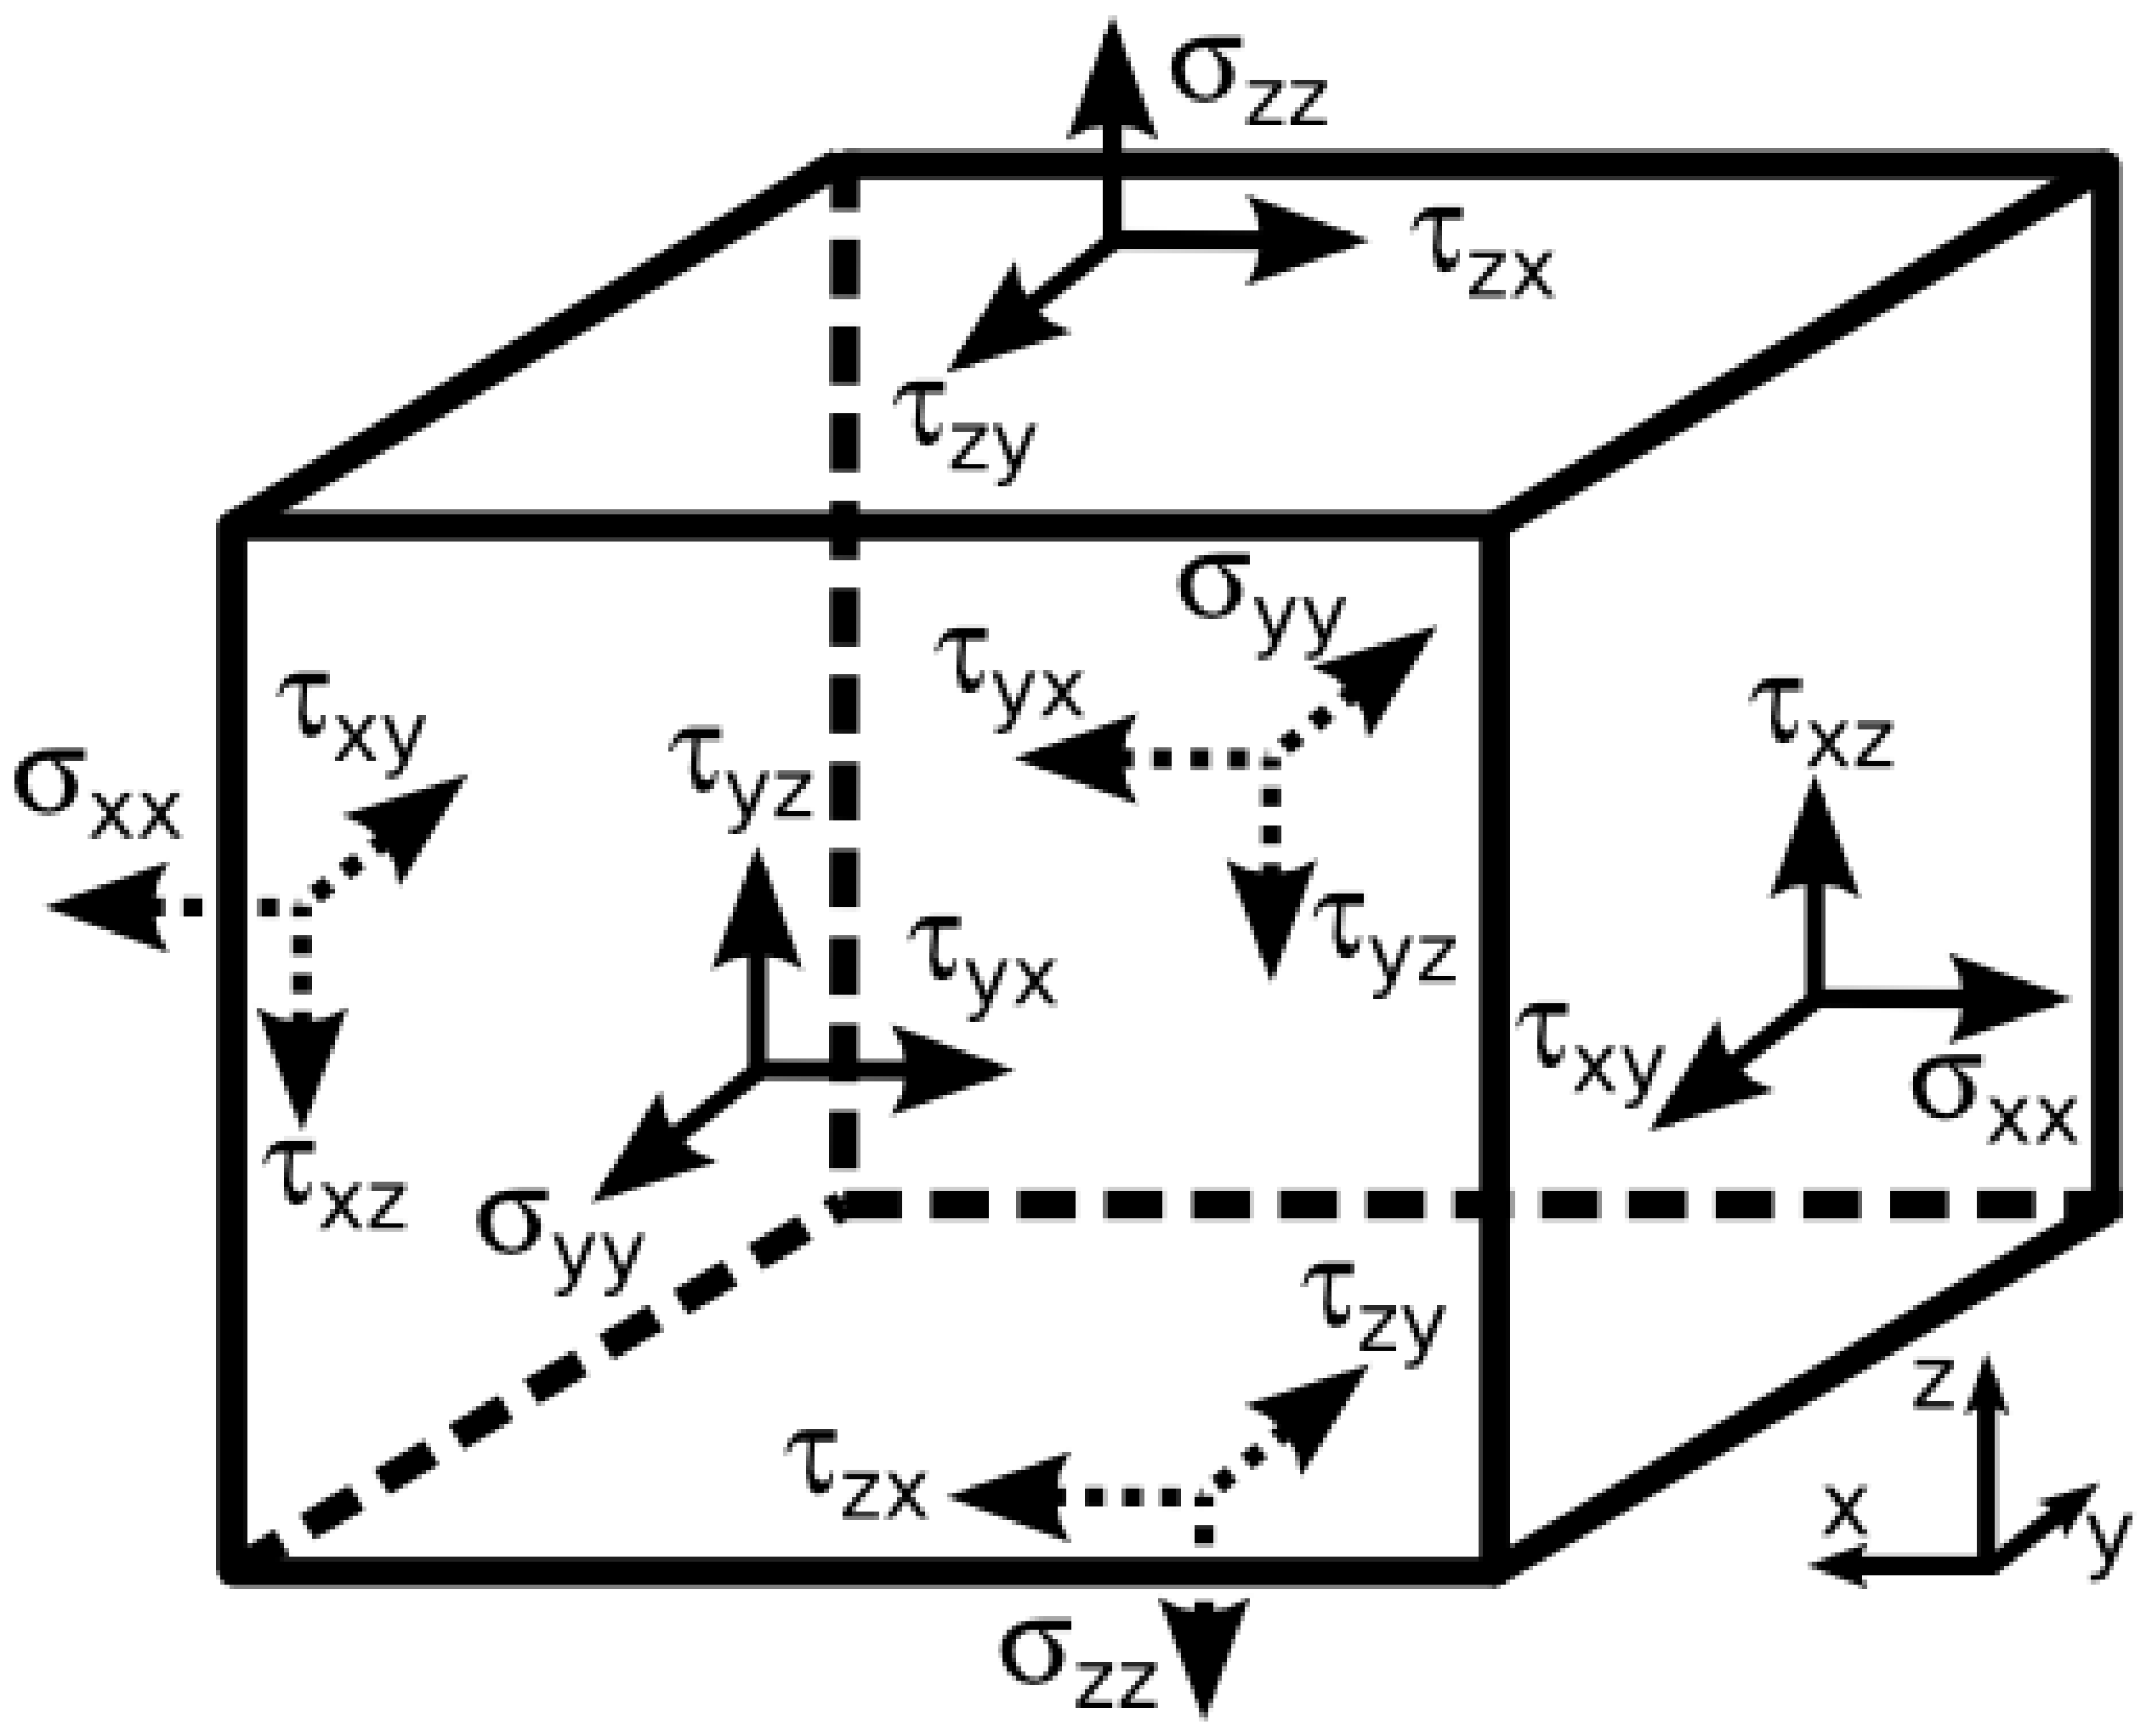
\includegraphics[scale=0.13]{images/stresses.eps}
  \caption{Složky viskózního napětí}
  \label{fig:stresses}
\end{center}
\end{figure} 

\noindent  Navíc pokud je daná tekutina izotropní (neupřednostňuje žádný směr deformace), tak tenzor \ref{eq:tenstress} má pouze šest nezávislých složek, protože mezi tečnými napětími platí vztahy:
\begin{equation}
    \begin{array}{ccc}
      \tau_{xy} = \tau_{yx}, & \tau_{xz} = \tau_{zx}, & \tau_{zy} = \tau_{yz}
      \end{array}
  	\label{eq:dept}
\end{equation} 
Pro Newtonovskou tekutinu dále platí, že jednotlivá viskózní napětí jsou úměrná míře lineárních deformací objemového elementu kontinua. Tenzor \ref{eq:tenstress} lze poté vyjádřit jako: 
\begin{equation}
    \vec{\vec{\tau}} = 
    \begin{bmatrix}
      2\eta\frac{\partial v_{x}}{\partial x} + \left( \lambda - \frac{2}{3} \eta  \right)  \nabla \cdot \vec{v} & \eta \left( \frac{\partial v_{x}}{\partial y} + \frac{\partial v_{y}}{\partial x} \right) & \eta \left( \frac{\partial v_{x}}{\partial z} + \frac{\partial v_{z}}{\partial x} \right)\\ 
      \eta \left( \frac{\partial v_{x}}{\partial y} + \frac{\partial v_{y}}{\partial x} \right) & 2\eta\frac{\partial v_{y}}{\partial y} + \left( \lambda - \frac{2}{3} \eta  \right)  \nabla \cdot \vec{v} 
      & \eta \left( \frac{\partial v_{y}}{\partial z} + \frac{\partial v_{z}}{\partial y} \right)\\ 
      \eta \left( \frac{\partial v_{x}}{\partial z} + \frac{\partial v_{z}}{\partial x} \right) & \eta \left( \frac{\partial v_{y}}{\partial z} + \frac{\partial v_{z}}{\partial y} \right)
      & 2\eta\frac{\partial v_{z}}{\partial z} + \left( \lambda - \frac{2}{3} \eta  \right) \nabla \cdot \vec{v}\\ 
    \end{bmatrix}
  	\label{eq:newtenstress}
\end{equation} 
Člen $\eta$ představuje dynamickou (tečnou) viskozitu a $\lambda$ značí dilatační (objemovou) viskozitu, jejíž hodnota je nulová pro jednoatomové plyny při nízké hustotě. Někdy se tenzor \ref{eq:newtenstress} zapisuje v úspornější podobě:
\begin{equation}
	\vec{\vec{\tau}} = \eta \left[ \nabla \vec{v} +  \left( \nabla \vec{v} \right)^{\mathsf{T}}\right] +  \left( \lambda -\frac{2}{3} \eta \right) \nabla \cdot \vec{v} \vec{\vec{I}}
	\label{eq:comptenstress}
\end{equation}
kde $\vec{\vec{I}}$ je jednotkový tenzor.

Dosazením vztahu \ref{eq:comptenstress} do rov. \ref{eq:cauchy} a při předpokladu nestlačitelnosti kontinua ($\nabla \cdot \vec{v} = 0$) se získá Navierova-Stokesova rovnice:
\begin{equation}
    \rho \left( \frac{\partial \vec{v}}{\partial t} + \vec{v} \cdot \nabla  \vec{v} \right) = -\nabla p + \eta \nabla^{2}\vec{v}  + \vec{f}
  	\label{eq:navst}
\end{equation} 
Ve trojrozměrné soustavě kartézských souřadnic lze vektorovou rov. \ref{eq:navst} rozepsat na 
\begin{equation}
\begin{array}{c}
    \rho \left( \frac{\partial v_{x}}{\partial t} + v_{x}\frac{\partial v_{x}}{\partial x} + v_{y}\frac{\partial v_{x}}{\partial y} + v_{z}\frac{\partial v_{x}}{\partial z} \right) = -\frac{\partial p}{\partial x} +  \eta \left( \frac{\partial^{2} v_{x}}{\partial x^{2}} + \frac{\partial^{2} v_{y}}{\partial y^{2}} + \frac{\partial^{2} v_{z}}{\partial z^{2}} \right) + f_{x}   \vspace{3mm} \\
    
    \rho \left( \frac{\partial v_{y}}{\partial t} + v_{x}\frac{\partial v_{y}}{\partial x} + v_{y}\frac{\partial v_{y}}{\partial y} + v_{z}\frac{\partial v_{y}}{\partial z} \right) = -\frac{\partial p}{\partial y} +  \eta \left( \frac{\partial^{2} v_{x}}{\partial x^{2}} + \frac{\partial^{2} v_{y}}{\partial y^{2}} + \frac{\partial^{2} v_{z}}{\partial z^{2}} \right) + f_{y}   \vspace{3mm} \\
    
    \rho \left( \frac{\partial v_{z}}{\partial t} + v_{x}\frac{\partial v_{z}}{\partial x} + v_{y}\frac{\partial v_{z}}{\partial y} + v_{z}\frac{\partial v_{z}}{\partial z} \right) = -\frac{\partial p}{\partial z} +  \eta \left( \frac{\partial^{2} v_{x}}{\partial x^{2}} + \frac{\partial^{2} v_{y}}{\partial y^{2}} + \frac{\partial^{2} v_{z}}{\partial z^{2}} \right) + f_{z}   \\
    \end{array}
  	\label{eq:navst3d}
\end{equation} 
Soustava rovnic \ref{eq:navst3d} spolu s rov. \ref{eq:conti1simp} tvoří systém čtyř parciálních diferenciálních rovnic pro neznámé $p$, $v_{x}$, $v_{y}$ a $v_{z}$. 

\subsection{Vícefázové modely}
Velké množství přírodních a průmyslových procesů je tvořeno vícefázovým prouděním. Problematika simulace tohoto děje je daleko komplexnější než v případě systému složeného pouze z jedné fáze. V hydrodynamice je pojem fáze chápán v širším smyslu než z termodynamického hlediska. Z tohoto pohledu lze fází definovat jako třídu materiálu, jenž interaguje určitým způsobem s dalšími částmi systému. 

V~současnosti existuje řada matematických modelů, které popisují vícefázové proudění a lišící se výsledným způsobem použití. Následující podkapitola obsahuje přehled modelů, které se nejčastěji využívají k~simulaci suspendace v~mechanicky míchaných nádobách. Především se jedná o simulační techniky Eulerian-Lagrangian, Eulerian-Eulerian a Eulerian-Granular.

\subsubsection{Model Eulerian-Lagrangian}
Tento typ modelu uvažuje primární tekutou fází jako kontinuum s~dispergovanou sekundární fází. Pro primární fázi je řešena rovnice kontinuity (\ref{eq:conti1simp}) spolu s~Navierovými-Stokesovými rovnicemi (\ref{eq:navst3d}), zatímco pro dispergovanou fázi je řešena trajektorie každé částice nebo skupiny částic separátně. Jednotlivé fáze si mohou mezi sebou vyměňovat hmotu, hybnost a energii, avšak vzájemné interakce částic mezi sebou jsou většinou zanedbány. Model Eulerian-Lagrangian je především vhodný pro systémy, kde objemový zlomek dispergované fáze nepřesáhne \SI{10}{\percent} např: rozprašovací sušárny, cyklóny nebo spalování uhlí či kapalného paliva. 

Řešením bilance sil působící na částici (rov. \ref{eq:dpm}) je získána její trajektorie v~daném časovém okamžiku.
\begin{equation}
	m_{p}\frac{d\vec{v}_{p}}{dt} = \vec{F}_{p} + \vec{F}_{g} + \vec{F}_{B} + \vec{F}_{D} + \vec{F}_{ad}
	\label{eq:dpm}
\end{equation} 
Členy $m_{p}$ a $\vec{v}_{p}$ na levé straně rov. \ref{eq:dpm} představují hmotnost částice a její vektor rychlosti. Pravá strana výše zmíněné rovnice obsahuje součet jednotlivých sil působících na diskrétní fázi. Symbol $\vec{F}_{p}$ značí sílu tlakového gradientu, jenž působí na částici vlivem akcelerace okolní kapaliny. Další členy $\vec{F}_{g}$ a $\vec{F}_{B}$ reprezentují gravitační resp. vztlakovou sílu. Jednotlivé příspěvky těchto sil lze rozepsat do tvaru:    
\begin{equation}
	\vec{F}_{p} + \vec{F}_{g} + \vec{F}_{B} = V_{p} \nabla p + m_{p} \vec{g} -  V_{p} \rho_{f} \vec{g}
	\label{eq:force3}
\end{equation} 
 Odporová síla $\vec{F}_{D}$ představuje výslednici sil kterou tekutina působí proti pohybu částic. Pro kulovou částici lze tento člen vyjádřit jako:
\begin{equation}
	\vec{F}_{D} = \frac{\pi}{8}C_{D}\rho_{f} d_{p}^{2} \left|\vec{v}_{p} - \vec{v}_{f}\right| \left(\vec{v}_{p} - \vec{v}_{f}\right)
	\label{eq:fd}
\end{equation} 
Bezrozměrné číslo $C_{D}$ v rov. \ref{eq:fd} se nazývá koeficient odporu nebo součinitel tření a vyjadřuje závislost odporu prostření na tvaru tělesa, charakteru proudění a vlastnostech tekutiny. Detailnějším rozborem tohoto členu se zabývá kapitola XXX.

Poslední příspěvkem $\vec{F}_{ad}$ do bilance \ref{eq:dpm} zahrnuje další síly působící na částici pevné fáze. Jedná se například o Saffmanovu vztlakovou sílu, jenž vzniká v důsledku vířivosti rychlostního pole kapalné fáze a působí především na částice o velikosti menší než několik mikrometrů. Další silou která se někdy zohledňuje při vícefázové simulaci je zdánlivá setrvačná síla, která je způsobena společným pohybem tekutiny v blízkosti dispergované fáze při její akceleraci. Tento jev má za následek dočasný zdánlivý nárůst hmotnosti částic. Zdánlivá setrvačná síla se projevuje především v systémech kapalina-plynná fáze.  

\subsubsection{Model Eulerian-Eulerian}
U~modelu Eulerian-Eulerian jsou jednotlivé fáze považovány za prostupující se kontinua a každý bod v~systému obsahuje informaci o~objemovém zlomku dané fáze. Z~tohoto popisu je zřejmé, že suma objemových zlomků přes všechny fáze v~libovolném bodě se vždy musí rovnat jedné. 
\begin{equation}
	\sum_{i=1}^n \alpha_{i} = 1
	\label{eq:volfrac}
\end{equation} 

Jednotlivé fáze mohou být kapalné, plynné nebo pevné a jejich celkový počet není teoreticky limitován. Pro každou fázi se řeší rovnice kontinuity a sada rovnic pro hybnost. K~výměně hybnosti mezi jednotlivými fázemi slouží mezifázové členy v~těchto rovnicích. Pokud dochází k~přenosu tepla nebo hmoty je třeba tuto skutečnost zohlednit v~bilanci energie a hmoty.    

Pro vícefázový systém je třeba zapsat rovnici kontinuity pro každou fázi zvlášť, přičemž je třeba obecně uvažovat přenos hmoty mezi jednotlivými fázemi. Rovnice kontinuity pro $i$-tou fázi lze zapsat jako:
\begin{equation}
	\frac{\partial}{\partial t} (\alpha_{i}\rho_{i}) +  \nabla \cdot (\alpha_{i}\rho_{i}\vec{v}_{i}) = \sum_{\substack{ i \neq j \\ j=1}}^{n}\Gamma_{ij}
	\label{eq:conti2}
\end{equation} 
kde člen $\Gamma_{ij}$ představuje hmotnostní tok mezi $i$-tou a $j$-tou fází vztažený na objemový element a $\alpha_{i}$ značí objemový zlomek dané fáze. Pokud však nedochází k transportu hmoty mezi fázemi, tak se rov. \ref{eq:conti2} zjednoduší do tvaru:
\begin{equation}
	\frac{\partial}{\partial t} (\alpha_{i}\rho_{i}) +  \nabla \cdot (\alpha_{i}\rho_{i}\vec{v}_{i}) = 0
	\label{eq:conti3}
\end{equation} 

Rovnice hybnosti pro $i$-tou fázi za předpokladu nulového mezifázového transportu hmoty lze zapsat jako:
\begin{equation}
	\frac{\partial}{\partial t} \left(\alpha_{i}\rho_{i}\vec{v}_{i}\right) + \nabla \cdot (\alpha_{i}\rho_{i} \vec{v}_{i} \otimes \vec{v}_{i}) = -\alpha_{i} \nabla p + \nabla \cdot \left(\alpha_{i} \vec{\vec{\tau}}_{i} \right) +\sum_{\substack{ i \neq j \\ j=1}}^{n} \vec{R}_{ji} + \vec{f}_{ext,i} + \vec{f}_{int,i}
	\label{eq:moml}
\end{equation}
\noindent kde $p$ je tlak sdílený mezi všemi fázemi, $\vec{\vec{\tau}}_{i}$ je tenzor viskózního napětí, jehož konkretní tvar závisí na typu uvažované fáze. Člen $\vec{R}_{ji}$ představuje mezifázovou odporovou sílu mezi $i$-tou a $j$-tou fází, $\vec{f}_{ext,i}$ má význam dalších objemových sil a $\vec{f}_{int,i}$ zahrnuje povrchové síly působící na $i$-tou fázi vlivem ostatních fází. Všechny výše zmíněné síly jsou vztaženy na objemový element dané fáze. 

Člen mezifázové odporové síly $\vec{R}_{ji}$ v~rovnici \ref{eq:moml} nejvýznamněji přispívá do popisu interakce mezi jednotlivými fázemi, a proto správnost popisu tohoto členu zásadně ovlivňuje kvalitu výsledné simulace. Tuto sílu lze rozepsat jakou součin koeficientu mezifázového sdílení hybnosti a relativní rychlosti $i$-té a $j$-té fáze.
\begin{equation}
	 \sum_{\substack{ i \neq j \\ j=1}}^{n} \vec{R}_{ji} = K_{ji} \left( \vec{v}_{j} - \vec{v}_{i} \right)
	\label{eq:kij}
\end{equation}
Z~definice \ref{eq:kij} je jasné, že platí vztah $\vec{R}_{ji} = -\vec{R}_{ij}$. Vzorec pro výpočet $K_{ji}$ se obecně liší podle toho jaké typy fází spolu interagují. Pokud se jedná o~interakci kapalina-pevná fáze, tak koeficient mezifázového sdílení hybnosti má tvar:
\begin{equation}
	K_{fs}= \frac{3\alpha_{s}C_{D}\rho_{f}\left|\vec{v}_{s} - \vec{v}_{f}\right|}{4d_{s}}
	\label{eq:kfs}
\end{equation}
Symbol $d_{s}$ značí průměr částic pevné fáze a $C_{D}$ je koeficient odpor, kterým se právě ovlivňuje chování odporové síly. 
 
Za zmínku stojí fakt, že při využití modelu Eulerian-Eulerian se pevná fáze modeluje jako kapalina bez vnitřního tření. Rigoróznější popis pevné fáze přináší až model Eulerian-Granular, který je diskutovaný níže. 

\subsubsection{Model Eulerian-Granular}
\label{sec:egm}
Vícefázový model Eulerian-Granular se liší od předchozího tím, že  popis chování pevné fáze byl odvozen s~využitím kinetické teorie, která je například známá ze statistického popisu plynů. U~tohoto modelu se viskozita pevné fáze mění v~závislosti na interakcích s~ostatními částicemi a primární fází. Mezi nejčastější aplikace patří simulace fluidních loží nebo suspendace v~mechanicky míchaných nádobách.

Bilanci hybnosti pro pevnou fázi $s$ má tvar:
\begin{equation}
	\frac{\partial}{\partial t} \left(\alpha_{s}\rho_{s}\vec{v}_{s}\right) + \nabla \cdot (\alpha_{s}\rho_{s} \vec{v}_{s} \otimes \vec{v}_{s}) = -\alpha_{s} \nabla p - \nabla p_{s} + \nabla \cdot \left(\alpha_{s} \vec{\vec{\tau}}_{s} \right) +\sum_{\substack{ j \neq s \\ j=1}}^{n} \vec{R}_{ji} + \vec{f}_{ext,s} + \vec{f}_{int,s}
	\label{eq:moms}
\end{equation}
Člen $p_{s}$ je tlak pevné fáze, který se skládá z kinetické části a členu, který výsledkem neelastických srážek mezi částicemi. V současnosti existuje řada modelů k výpočtu tlaku pevné fáze. Jedním z nich je model odvozený autory \citet{lun84}:
\begin{equation}
	p_{s} = \alpha_{s}\rho_{s}\Theta + 2\rho_{s}\left(1 + r_{s} \right) \alpha_{s}^{2}g_{s}\Theta
	\label{eq:ps}
\end{equation}
kde $r_{s}$ je restituční koeficient vyjadřující míru elasticity srážek mezi částicemi. Symbol $g_{s}$ představuje radiální distribuční funkci, jenž upravuje pravděpodobnost kolizí částic pevné fáze. Poslední nediskutovaným členem $\Theta$ je teplota zrnité fáze, která je úměrná velikosti střední kvadratické rychlosti náhodného pohybu částic, tedy: 
\begin{equation}
	\Theta = \frac{1}{3}\left< \vec{u} \cdot \vec{u} \right>
	\label{eq:gtemp}
\end{equation}
Ve většině CFD řešíčů se určení hodnoty teploty zrnité fáze využívají algebraické modely odvozené z transportní rovnice pro tuto veličinu.

Tenzor viskózního napětí pevné fáze $\vec{\vec{\tau}}_{s}$ v rov. \ref{eq:moms} lze vyjádřit formálně stejně jako ve vztahu \ref{eq:comptenstress}. 
\begin{equation}
	\vec{\vec{\tau_{s}}} = \eta_{s} \left[ \nabla \vec{v_{s}} +  \left( \nabla \vec{v_{s}} \right)^{\mathsf{T}}\right] +  \left( \lambda_{s} -\frac{2}{3} \eta_{s} \right) \nabla \cdot \vec{v_{s}} \vec{\vec{I}}
	\label{eq:solidstress}
\end{equation}
Tečná viskozita zrnité fáze $\eta_{s}$ je dána součtem kolizní, kinetické a frikční části:
\begin{equation}
	\eta_{s} = \eta_{s,col}  + \eta_{s,kin} + \eta_{s,fr} 
	\label{eq:nys}
\end{equation}
přičemž běžně využívané korelace k jejich určení byly navrženy \citet{gid92}, \citet{syam93}. Dilatační viskozita $\lambda_{s}$ zohledňuje odpor pevných částic při expanzi či kompresi. \citet{lun84} odvodili následující vztah k jejímu výpočtu:
\begin{equation}
	\lambda_{s} = \frac{4}{3}\alpha_{s}\rho_{s}d_{s}g_{s}\left(1 + r_{s} \right)\sqrt{\frac{\Theta}{\pi}}
	\label{eq:dilvis}
\end{equation}
 
\subsection{Odporový koeficient}
V~současnosti existuje řada modelů pro koeficient odporu, které se liší podle toho pro jaký účel byly navrženy. Jedním z~nejznámějších je model, který navrhli \citet{schi32}. Autoři získali vztah \ref{eq:schlneu} pro výpočet koeficientu odporu na základě experimentálního měření rychlosti usazování sférické částice ve stagnantním sloupci kapaliny.    
 
	\hypertarget{hyp:schlneu}{} 
\begin{equation}
	\label{eq:schlneu}
  C_{D0} = \left\{ \begin{array}{ll}
  \frac{24}{Re_{p}}  \left( 1 + \num{0.15}Re_{p}^{\num{0.687}} \right) & Re_{p} \le 1000\\
  \num{0.44} & Re_{p} > 1000\\
  \end{array} \right.
\end{equation}

\noindent Ze vztahu \ref{eq:schlneu} je patrné, že Schillerova-Naumannova korelace je funkcí Reynoldsova kritéria pro částici které je definováno jako:

\begin{equation}
	Re_{p}= \frac{\rho_{f}d_{s}|\vec{v}_{s} - \vec{v}_{f}|}{\eta_{f}}
	\label{eq:reyp}
\end{equation}

Bohužel koeficient odporu navržený Schillerem a Naumannem se ukázal jako nepříliš vhodný k~popisu odporové síly v~systémech s~plně vyvinutým turbulentním prouděním. Proto řada autorů navrhla úpravu této korelace a některé z~nich jsou uvedeny v~tab. \ref{tab:cds}. Člen $\lambda$ se nazývá Kolmogorovo mikroměřítko a určuje nejmenší velikost turbulentní vírů přítomných v~systému, přičemž je funkcí kinematické viskozity a disipace energie.

\begin{table}[h!]
\begin{center}
  
		\hypertarget{hyp:cds}{}
		\caption{Modely pro odporový koeficient v~turbulentní oblasti proudění}
		\label{tab:cds}
\begin{tabular}{|c|c|>{\centering\arraybackslash}p{5cm}|}
  \hline
  
{\textbf{Autor}} & {\textbf{Koeficient odporu}} & {\textbf{Stanoveno na základě}} \\ \hline{}

\citet{pin01} & $C_{D} = C_{D0} \left( \num{0.4}\tanh\left(  \frac{16\lambda}{d_{s}} - 1  \right) \right) ^{-2}$ & měření rychlosti usazování v~míchací nádobě \\ \hline
 
\citet{bru98} & $C_{D} = C_{D0} \left( 1 + \num{8.76e-4} \left( \frac{\lambda}{d_{s}} \right)^{3} \right)$ & experimentální studie Taylorova–Couetteova toku \\ \hline 

\citet{kho06} & $C_{D} = C_{D0} \left( 1 + \num{8.76e-5} \left( \frac{\lambda}{d_{s}} \right)^{3} \right)$ & úpravy Brucatova vztahu pro míchací nádoby  \\ \hline 

\end{tabular}
\end{center}
\end{table}